\section{Sicherheitsarchitektur iOS}
	\subsection{Secure boot chain}
	Apple hat eine Kette aneinander gereihter, vom Vorgänger abhängiger Prozesse
	entwickelt, um den Startvorgang möglichst abzusichern und eine Manipulation
	der Low-Level Software auszuschließen. Dieses "`secure boot chain"'
	genannte Verfahren stellt sicher, dass iOS nur auf Geräten startet, welche
	auf diesem Wege erfolgreich validiert wurden. Dabei wird nach dem Start
	eines iOS Gerätes zuerst Code aus einem nur lesbaren Speicherbereich
	ausgeführt. Dieser hardware of trust genannte unveränderbare Code ist bei
	der Manufaktur der Chips eingebettet worden und somit implizit vertraulich. 
	Das Boot ROM enthält zusätzlich Apple's öffentlichen Schlüssel des Root 
	Zertifikats, welcher sicher stellt, dass der Low-Level-Bootloader von Apple 
	signiert ist, bevor er ausgeführt wird.
	
	%\begin{figure}[h]
		%\centering
 		%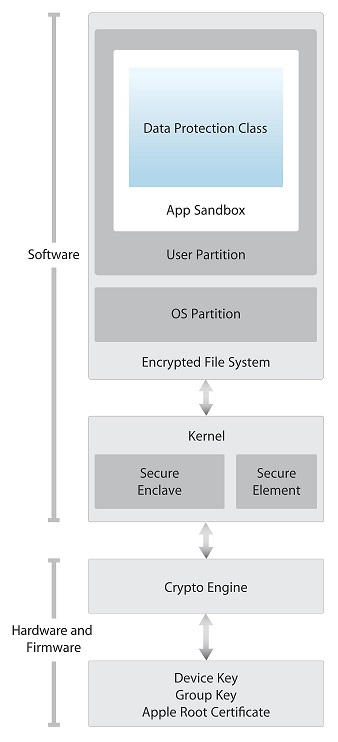
\includegraphics[width=0.3\linewidth]{ios/media/security-model.jpg}
        %\caption{Sicherheitsarchitektur Diagramm von iOS}
        %\label{fig:security-model}
    %\end{figure}\\
    %ref: Figure \ref{fig:security-model} shows the sec. arch.
    
    %\begin{wrapfigure}[Zeilen]{Position}[Ueberhang]{Breite}
	\begin{wrapfigure}[0]{r}[0.5cm]{6cm}
		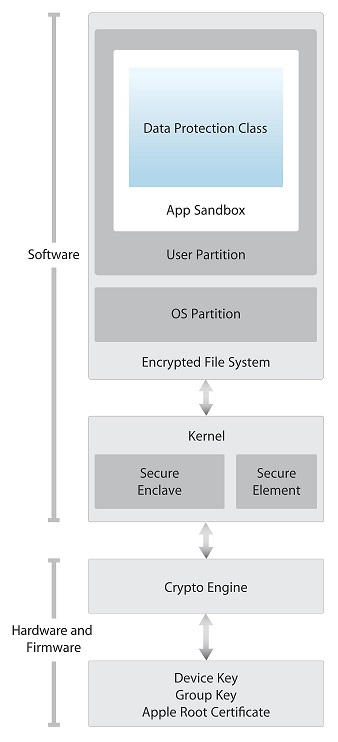
\includegraphics[width=\linewidth]{ios/media/security-model.jpg}
		\caption{Sicherheitsmodel von iOS}
		\label{fig:security-model}
	\end{wrapfigure}
	\subsection{iOS Sicherheitsmodel}
	Apple integrierte vier Schichten der Sicherheit in iOS.\\